\documentclass[a4paper, twoside]{report}

\usepackage[english]{babel}
\usepackage[utf8x]{inputenc}
\usepackage[T1]{fontenc}
\usepackage{listings}
\usepackage{hyperref}
\hypersetup{colorlinks=false}
\usepackage{lscape}
\usepackage{subfigure}
\usepackage{amsmath}
\usepackage{graphicx}
\usepackage[colorinlistoftodos]{todonotes}
\usepackage{setspace}
\usepackage{subcaption}

\onehalfspacing
%% Sets page size and margins
\usepackage[a4paper,top=2cm,bottom=2cm,left=3cm,right=3cm,marginparwidth=1.75cm]{geometry}

\title{Metamaterials, Non-affine Deformations and Deployable Structures}
\author{Apoorv Srivastava}
% Update supervisor and other title stuff in title/title.tex

\begin{document}
\begin{titlepage}

\newcommand{\HRule}{\rule{\linewidth}{0.5mm}} % Defines a new command for the horizontal lines, change thickness here

%----------------------------------------------------------------------------------------
%	LOGO SECTION
%----------------------------------------------------------------------------------------

\center\includegraphics[width=8cm]{title/logo.png}\\[1cm] % Include a department/university logo - this will require the graphicx package
 
%----------------------------------------------------------------------------------------

\center % Center everything on the page

%----------------------------------------------------------------------------------------
%	HEADING SECTIONS
%----------------------------------------------------------------------------------------
\quad\\[1.5cm]
%\textsc{\LARGE MSc Thesis}\\[1.5cm] % Name of your university/college
\textsc{\Large IIT Bombay}\\[0.5cm] % Major heading such as course name
\textsc{\large Department of Civil Engineering}\\[0.5cm] % Minor heading such as course title

%----------------------------------------------------------------------------------------
%	TITLE SECTION
%----------------------------------------------------------------------------------------
\makeatletter
\HRule \\[0.4cm]
{ \huge \bfseries \@title}\\[0.4cm] % Title of your document
\HRule \\[1.5cm]
 
%----------------------------------------------------------------------------------------
%	AUTHOR SECTION
%----------------------------------------------------------------------------------------

\begin{minipage}{0.4\textwidth}
\begin{flushleft} \large
\emph{Submitted by:}\\
\@author \\ % Your name\\
(160040081)
\end{flushleft}
\end{minipage}
~
\begin{minipage}{0.4\textwidth}
\begin{flushright} \large
\emph{Supervisor:} \\
Prof. Mandar M. Inamdar
% Uncomment the following lines if there's a co-supervisor
%\\[1.2em] % Supervisor's Name
%\emph{Co-Supervisor:} \\
%Dr. Adam Smith % second marker's name
\end{flushright}
\end{minipage}\\[3cm]
\makeatother


%----------------------------------------------------------------------------------------
%	DATE SECTION
%----------------------------------------------------------------------------------------

{\large BTP Report}\\[0.5cm]

{\large \date{}}\\[2cm] % Date, change the \today to a set date if you want to be precise

\vfill % Fill the rest of the page with whitespace

\end{titlepage}

\begin{abstract}
Deployable Structures are the structures which can be collapsed into compact modules and deployed when needed. While unlike their static counterparts, these structures are not ubiquitous, some examples of deployable structures present around us are Umbrellas, Scissors and foldable furniture such as tables and chairs. Affine deformations are deformations are the deformations which translate uniformly at the microscopic level and can be defined using linear translations and rotations, following this, non-affine deformation are the deformations which do not translate linearly from microscopic to macroscopic level owing to the topology of the materials. Coupling the ideas or non-affine deformations and deployable structure at microscopic level leads to design of materials having special properties and such materials are called metamaterials. In addition to these, the project involved study of Mechanism, Lattices, Origami and Topological Mechanics.

The later half of the project involved modelling the plates using the spring ball models and benchmarking the results with analytical theories. This was done in order to develop a program which can accurately model plates, following which study of the effect of pre-stress in the springs on the properties of the plate can be carried out. This will help in determining strain fields which will result in plate deforming to a specified shape and the ways in which pre-stress affect the dynamic properties of plate. An added advantage of such modelling is that it can be used to predict the plate displacements and following that stresses in the plate for complex loading and cases where theoretical results are not available or are difficult to arrive at.


\end{abstract}

\renewcommand{\abstractname}{Acknowledgements}
\begin{abstract}
I would like to thank Prof. Mandar. M. Inamdar for connecting me to all these fascinating topics and insightful discussions which proved to be of great help in understanding these topics. I feel extremely privileged to be his student. I would also like to thank Kshitij Vijaywargiya for initially uncovering the idea of deployable structures for me. 

Special thanks to my wing mates for being a constant source of entertainment, everytime I was stressed.
\end{abstract}

\tableofcontents
\listoffigures

\chapter{Introduction}
The project is aimed towards the study of novel structure and materials at macro as well as micro level, understanding their structure and behavior, and ways in which they can altered to achieve required functionalities. The project started with the study of deployable structures and eventually diverged to touch several exciting fields which are described below. 


Following the introduction to these ideas, a spring ball model for plate was developed, with the aim of understanding the effects of pre-stress and non-homogeneous strain fields on the deformed shape and properties of the plate. The system could model non-homogeneous strain field and non-uniform expansion and contraction (due to uneven temperature fields) by varying the natural length of the springs in the model.

\section{Deployable Structure}
Deployable structures are defined as the structures capable of undergoing large changes in shape. These structures are also often referred to as foldable, reconfigurable, auxetic, extendible or expandable structures. Deployable structures are used extensively in the Aerospace industry where large structures such as satellites, antennas, solar arrays etc need to be packaged in compact volumes and deployed when in outer space. Typically, deployable structures are used for ease of storage and transportation, and they are deployed into their operational configuration when required. Some day-to-day examples of deployable structure observed around us are umbrella and folding chairs. An essential requirement for deployable structures is that the transformation should be possible without any damage, and should be reliable.

There are two manners in which development of deployable structure is undertaken. The first one involves the use of structural components, the components may be rigid or flexible or combination of both. In this approach the deployment process is fully controlled and the structure is stable at all stages of deployment. Due to the higher durability of structural components, these kind of structures have applications in architecture as well. Such deployable structures are further classified into Rigid (Scissors, NASA type cubic, \href{https://en.wikipedia.org/wiki/Bengt_Sjostrom_Theatre}{Bengt sjostrom starlight theatre}), Deformable (Inflatable air cell structures), Flexible (Fast Mast), and Combined systems (Retractable memberanes). The second approach employs generative techniques such as origami, biomimetics and other form inspiring sources. This approach not only informs the design of macro-structures but is also helping researchers develop materials with novel properties. The generative technique is further classified into Origami paper pleat (Origami Bags, Two way fold trusses) and Biomemetics (Wing folding in beatles, geometry of unfolding leaves). \cite{rivas2015deployable} \cite{Filip} \cite{Zha}
 
\begin{figure}[htbp]
    \centering
    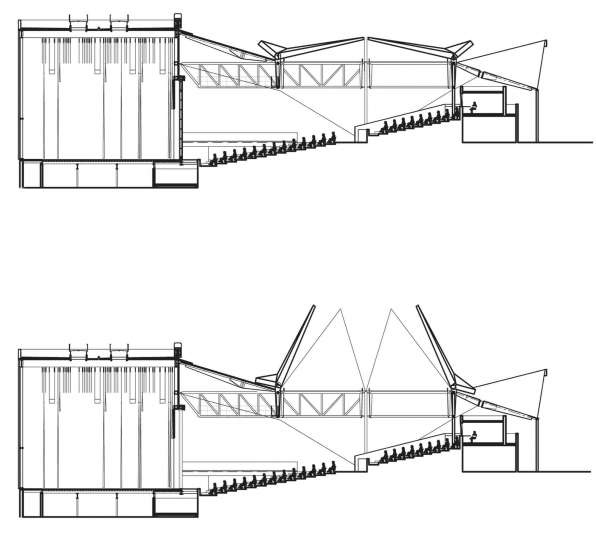
\includegraphics[width = 0.8\linewidth]{Figures/Bengt_theatre.jpg}
    \caption{Schematic Diagram of Bengt sjostrom starlight theatre, Image credit: www.archdaily.com}
    \label{fig:Bengt_theatre}
\end{figure} 

According to Maxwell's Lemma, the lightest (and therefore most efficient) structure separates compressive and tensile elements, this leads to a special class of Deployable structures called Tensegrity, Tensional integrity or Floating compression. Such structures consist of compression members floating in a net of tension members and the compression members do not usually touch each other. Since there is no bending, such structures are extremely efficient and have high rigidity-to-weight ratio. \cite{pellegr}

\section{Mechanisms and States of self stress}
Pin jointed frameworks can be classified into truss and mechanisms based on their connectivity. While a truss is defined as a rigid structure capable of carrying loads when simply supported, according to classical definition, Mechanism is defined as a system of rigid elements connected through pins and joints capable of movement. These mechanisms are classified into several groups such as planar mechanisms, spatial mechanisms, spherical mechanisms and so on. This classification can also be examined in terms of Static and Kinematic Indeterminacy.\cite{Pelle}


The assemblies in which all member forces can be determined using the equations of equilibrium are classified as statically determinate structure. Another equivalent definition of static determinacy is that for a given system, the number of equations is equal to the number of unknowns and the coefficient matrix is non-singular. Similarly Kinematic determinate structures are the assemblies in which the position of the nodes can be determined exactly (on one side of the base plane) based on the lengths of bars. kinematically indeterminate structures are the assemblies in which position of nodes can not be determined uniquely and they have one or more mode of inextensional deformation. It means that such an assembly can distort without change in member lengths which essentially makes it a mechanism. In a similar manner, state of self stress is related to statically indeterminate structures. When an assembly has states of self stress, it's member can have forces without application of any external load. 

Deployable structures generated using mechanisms belong to the structural class. While the Maxwell's rule provides condition for the static and kinematic determinacy based on the equality of number of equations and number of unknowns when structure is adequately connected to the foundation as 
\begin{equation}
    b = dJ,
\label{eq:cacona}
\end{equation}

\noindent where b is the total number of bars, d is dimension of the problem and J is the number of non foundation joints.

However, exceptions exist to this rule in form of structures which satisfy Maxwell's rule but still are kinematically indeterminate.

A more exhaustive treatment of equilibrium and kinematic matrix provides a more complete explanation for these anomalies.

The equilibrium matrix of a structure is a $(3j - k)$ by $b$ matrix which relates the member tensions $\boldsymbol{t}$ with external loads $\boldsymbol{f}$ as
\begin{equation}
    \boldsymbol{A.t = f}
    \label{eq:cacona}
\end{equation}
\noindent where j is total number of joints, k is number of kinematic constraint on foundation joints and b is the total number of bars.

In a similar manner, for small deformations, member elongations $\boldsymbol{e}$ and displacements of joints $\boldsymbol{d}$ can be related using a $b$ by $(3j - k)$ matrix $\boldsymbol{B}$ as
\begin{equation}
    \boldsymbol{B.d = e}
    \label{eq:cacona}
\end{equation}

\noindent Using the principle of virtual work, one can show that $\boldsymbol{B = A^T}$. The fundamental sub-spaces associated with these matrices and there significance are as following:

\begin{enumerate}
    \item \textit{Column Space of A} : Provides the range of $\boldsymbol{f}$ that can be supported by the structure and modes of displacement that require elongation of one or more bars.

    \item\textit{Left nullspace of A} : Describes the range of $\boldsymbol{f}$ that can not be supported by the structure in its original configuration and it is the space spanned by inextensional mechanisms.

    \item\textit{Row Space of A} : Spans the space generated by bar tensions in equilibrium with the applied load and describes geometrically compatible bar elongations.

    \item\textit{Nullspace of A} : represents sets of tension which are in equilibrium with zero loads (states of self stress) and bar elongations forbidden by the geometry.
\end{enumerate}



The analysis of these sub-spaces associated with the matrices $\boldsymbol{A}$ and $\boldsymbol{B}$ results in modified Maxwell's equation as
\begin{equation}
    s = b - r_{A},  \hspace{1cm} m = 3j - k - r_{A},
    \label{eq:cacona}
\end{equation}
\noindent subtracting two equations we get
\begin{equation}
    s - m = b - 3j + k
    \label{eq:cacona}
\end{equation}
\noindent here s is the number of states of self stress, and m is the number of mechanisms present in the structure. $r_{A}$ is the rank of the matrix A.

Further investigation of these matrices provides us with a way to distinguish between finite and infinitesimal mechanisms. These insights coupled with the interpretation of fundamental sub-spaces provide the information necessary for design of mechanism based deployable structures\cite{Pelle}.


\section{Origami}
Origami is a Japanese word derived from ori meaning "folding", and kami meaning "paper" and stands for the art of paper folding. Another term closely associated with Origami is Kirigami, unlike origami cutting of the paper is allowed in Kirigami. The Origami technique comprises of several basic basic folds like valley and mountain folds, pleats, reverse folds, squash folds, and sinks, which are used to generated complex patterns and shapes using a single sheet of paper.


The art of Origami has found several applications in the industries such as medical and space industry and continues to inspire new techniques in other fields. The techniques of origami are currently being investigated for development of new materials and tools such as Metamaterials, Sandwich panels, drones and robots.

Origami aids in the development of deployable structures through the generative pathway\cite{rivas2015deployable}. Origami provides a way to pack the structures into compact spaces. The origami models can be morphed into real structure by developing the equivalent bar and hinge models\cite{FilipBarandHinge}. The simplicity of such models make them well suited for the engineering community, and their efficiency make them suitable for design problems such as optimization and parameterization of geometric origami variations.The application of origami for development of deployable structures can be best illustrated by examples as shown in the Fig~\ref{fig:OrigamiEx}.
\begin{figure}[htbp]
    \centering
    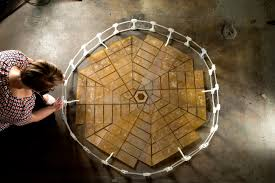
\includegraphics[width = 0.8\linewidth]{Figures/Origami_NASA.jpg}
    \caption{Origami based deployable solar panel for space application, Image credit: NASA}
    \label{fig:OrigamiEx}
\end{figure}


Furthermore the concepts of origami combined with the metamaterials provide a way for the structures which follow different energy pathways during deployment and contraction, which makes them highly desirable since they can be designed to resist immediate collapse by providing an energy barrier in their contraction pathway\cite{Zha}. This also adds to the reliability for use of deployable structures making their stability less dependent on locking mechanisms. In addition to this Origami can also be used for programming curvatures\cite{Dud}, and development of metamaterials\cite{Filip}.

In simple cases of pure origami based deployable hollow triangulated cylinders, based on the energy required the structures can be classified as easy-deploy-easy-collapse (requiring no or minimal energy for deployment as well as collapse) or hard-deploy-hard-collapse (requiring significant amount of energy for deployment as well as collapse). Easy-deploy-easy-collapse structures generate minimal strain in members of their equivalent bar and hinge model while hard-deploy-hard-collapse structure create large strains leading to even failure in case of conventional materials\cite{Zha,FilipBarandHinge}. The tubes can be designed to fall in one of the types by varying simple parameters which is shown in the next chapter.

\section{Mechanical Metamaterials}
Metamaterials are defined as the materials which are engineered for the properties that are not present in naturally occurring materials. Metamterials gain their property from their internal structure and connectivity rather than the materials properties. Based on the property with which a metamaterial is concerned, it is classified into one of the several sub-divisions such as Electromagnetic Metamaterials, Thermo-Electric Metamaterials and so on. Mechanical metamaterials are concerned with mechanical properties of matter and focuses on achieving unusual values for mechanical parameters such as density, Poisson's ratio, and compressibility. Recent development in the field are associated with the development of exotic functionalities such as pattern and shape transformation in response to mechanical forces, unidirectional guiding of motion and waves and reprogrammable stiffness\cite{Berto, Surj}.

The domain of metamaterials which deals with materials having tunable stiffness forms a connection between metamaterials and deployable structure. Simplest instance of use of metamaterials in deployables is in the structures which have different energy paths for deployment and collapse, as explained earlier. Using a conventional material, if an element experiences compression during the process of deployment, it will experience tension while collapsing and usually the stiffness in tension as well as compression is same for materials and thus energy path followed is same for two deployment as well as collapse, however for material which exhibit different stiffness for tension and compression will have different profiles for two process and can lead to structures which deploy easily but offer resistance for collapsing and vice versa.\cite{Zha} 

Furthermore soft metamaterials and materials at the verge of instability have parameters which can be tuned to develop hinges and joints as part of elements engendering the possibility of a unified deployable systems without any external joints.\cite{Baardink489, Rock}

Design of metamaterials also draws from Origami, Mechanism, Topology, and form finding making a cohesive whole of all these ideas\cite{Filip, Rock}.

\section{Form Finding}
The primary motive of the form-finding process is to identify the geometry that sustains the load coming on the structure most efficiently or the shape a structure takes under a given load. In cases when elasticity and geometric constraints are intertwined, for example structure such as elastic gridshells which buckle by design, actuated shapes are difficult to predict using classical methods. Such cases suggest the presence of multi-stable states and the analysis requires inclusion of higher modes of the structure. Such techniques can applied in the opposite direction as well to determine the boundary conditions and forces that need to be applied on the structure to achieve the desired shape.\cite{Baek75} 

The ideas of form finding are usually applied in the reverse direction to determine the boundary conditions which will lead to the structure taking the desired shape. The deformations involved are usually large and material needs to be elastic during the entire process so that the structure can be deployed and collapsed a number of times, this provides another entry point for the application of metamaterials.

An example where this relationship is elicited is that of form finding in elastic gridshells. Initially planar elastic grid is actuated into a shell like structure by loading their extremities. It was observed that the resulting shapes are complex even for simple configuration and indicated the presence of multi-stable states and higher order modes in the actuated grid. However it is possible to parameterize these complex shape and by varying these parameters desired actuated shape can be obtained\cite{Baek75}.

\section{Elastic Bilayers}
Elastic Bilayers stands for shape shifting thin sheets made up of active materials that respond to stimuli such as heat, light and humidity. Such layers are designed by solving the geometric inverse problem of determining the growth factors and directions for a given isotropic elastic bilayer to grow into a target shape by posing and solving an elastic energy minimization problem. Such techniques aid in engineering complex functional shapes in tissues, and actuation systems in soft robotics.\cite{va}

In general nonuniform in-plane growth of thin sheets results in out of plane buckling. This process is responsible for several process in nature such as shaping of leaf and blooming of flowers. Generally, such sheets settle in residually strained configuration which is a local minima of the energetic cost of stretching and bending the sheet. Since it's a local minima, this state might not be unique. By solving the inverse problem one can design the layer such that it can be used to achieve any target surface shape from any reference shape\cite{va}. Similar to the case of form finding, this involves parameterizing the surface and solving the inverse problem.

\section{Topological Mechanics}
In Mathematics, Topology is defined as the study of properties of a geometric object that are preserved under continuous deformations, such as stretching, twisting, crumpling and bending. The concepts from Topology are aiding the development of novel materials such as topological insulators, and topological photonics. In the recent times, the concepts from electronic topological states are being applied to mechanics to identify topological mechanical properties. Topological mechanics encompasses the study of topological phonon modes of the material, which has applications in development of mechanical insulators and metamaterials with topologically protected mechanical properties.\cite{Ma, Rock, Baardink489, Che}

Topology involves the study of connectivity of different elements in a system and is essential to the idea of deployable structures. Topology plays an important role in determining the member connectivity in deployable trusses and folding motions of Origami and Kirigami\cite{Che}.

In addition to the deployable structures, It has a huge role in development of metamaterial\cite{Rock, Berto, Surj} and lattice mechanics\cite{Ma}. Topology can be used to control the mechanical properties of a material along an edge or around a localized defect, topological polarization of a network governs along with its variation and orientation define the rigidity of the network. The topology of the lattices can be varied to move between states with dramatically varying mechanical properties such as elastic modulus, wave characteristics and so on. 

\section{Lattices \& Non-Affine Deformations}
Lattice is an ordered arrangement of particles which repeats infinitely in all dimensions of the lattice. The unit cell of a lattice is defined as the smallest repeating unit having the full symmetry of the lattice and Structure of a lattice is described by its unit cell. A lattice may have more than one unit cell which when translated can generate entire lattice. A special class of lattices are termed as Maxwell lattices. Maxwell lattices are mechanical frames having average coordination number equal to twice their spatial dimension, this leaves them on verge of mechanical instability. Fourier Transform of these lattices also results in lattices, which are called Reciprocal Lattices and present the lattice in reciprocal space. Reciprocal Lattices are used for determining the phonon modes which helps in design of materials with topologically protected material properties.


Changes in the metric properties of a continuous body is defined as deformation, this indicates that a curve drawn on original body will change its length after the body is deformed. Usually deformations are affine which means that the deformations can be described in terms of affine transformation, or equivalently local strain in a sample after deformation is identical everywhere and equal to the macroscopic strain. All deformations other than affine deformations are termed as non-affine deformation. One of the principal sources of non-affinity is a space or time dependent elastic constant. The local environment in a disordered solid varies in space, depending crucially on local connectivity or coordination such that the local displacement $\textbf{u}$ may not be simply related to the applied stress $\boldsymbol{\sigma}$. Such non-affine displacements are present even at zero temperature, are material dependent, and vanish only for homogeneous crystalline media without defects\cite{Gang}.

The deployable structure connects with the lattices at two level, on a trivial level, the lattices can be considered as a special kind of structure and mechanisms involved in such structures connect them directly with the ideas of deployable structure. Lattices require special attention owing to their periodic boundary conditions. Depending on the topology of lattice, actuation may propagate throughout the lattice or may cease within a few unit cells \cite{Neli}. Furthermore, it can be shown that static determinacy and kinematic determinacy can not exist in these structures concurrently \cite{Gues}. 

On a more elaborate level, Metamaterials connect the deployable structures with lattices since design of metamaterials requires realization and application of lattice mechanics and properties which is ultimately utilized for development of deployable structures. Lattice mechanics is essential to the development of metamaterials with unusual elastic modulus and phonon gaps.\cite{Ma}


\chapter{Connecting The Dots...}
While the concepts mentioned in the previous chapter might seem disparate at first, they are closely related with one other and each of them follows naturally from the preceding one. This chapter is aimed at eliciting the flow between these topics. 

While the background theme of the project is deployable structures, this gradually diverged to encompass several ideas mentioned in the first chapter.

\section{Deployable Structures and Mechanisms}
As mentioned earlier, there are two approaches taken for development of deployable structure, namely structural components and generative techniques. The concepts of mechanisms come in the picture through the first way. 

While the Maxwell's rule provides condition for the static and kinematic determinacy based on the equality of number of equations and number of unknowns when structure is adequately connected to the foundation as 
\begin{equation}
    b = dJ,
\label{eq:cacona}
\end{equation}

\noindent where b is the total number of bars, d is dimension of the problem and J is the number of non foundation joints.

However, exceptions exist to this rule in form of structures which satisfy Maxwell's rule but still are kinematically indeterminate.

A more exhaustive treatment of equilibrium and kinematic matrix provides a more complete explanation for these anomalies.

The equilibrium matrix of a structure is a $(3j - k)$ by $b$ matrix which relates the member tensions $\boldsymbol{t}$ with external loads $\boldsymbol{f}$ as
\begin{equation}
    \boldsymbol{A.t = f}
    \label{eq:cacona}
\end{equation}
\noindent where j is total number of joints, k is number of kinematic constraint on foundation joints and b is the total number of bars.

In a similar manner, for small deformations, member elongations $\boldsymbol{e}$ and displacements of joints $\boldsymbol{d}$ can be related using a $b$ by $(3j - k)$ matrix $\boldsymbol{B}$ as
\begin{equation}
    \boldsymbol{B.d = e}
    \label{eq:cacona}
\end{equation}

\noindent Using the principle of virtual work, one can show that $\boldsymbol{B = A^T}$. The fundamental sub-spaces associated with these matrices and there significance are as following:

\begin{enumerate}
    \item \textit{Column Space of A} : Provides the range of $\boldsymbol{f}$ that can be supported by the structure and modes of displacement that require elongation of one or more bars.

    \item\textit{Left nullspace of A} : Describes the range of $\boldsymbol{f}$ that can not be supported by the structure in its original configuration and it is the space spanned by inextensional mechanisms.

    \item\textit{Row Space of A} : Spans the space generated by bar tensions in equilibrium with the applied load and describes geometrically compatible bar elongations.

    \item\textit{Nullspace of A} : represents sets of tension which are in equilibrium with zero loads (states of self stress) and bar elongations forbidden by the geometry.
\end{enumerate}



The analysis of these sub-spaces associated with the matrices $\boldsymbol{A}$ and $\boldsymbol{B}$ results in modified Maxwell's equation as
\begin{equation}
    s = b - r_{A},  \hspace{1cm} m = 3j - k - r_{A},
    \label{eq:cacona}
\end{equation}
\noindent subtracting two equations we get
\begin{equation}
    s - m = b - 3j + k
    \label{eq:cacona}
\end{equation}
\noindent here s is the number of states of self stress, and m is the number of mechanisms present in the structure. $r_{A}$ is the rank of the matrix A.

Further investigation of these matrices provides us with a way to distinguish between finite and infinitesimal mechanisms. These insights coupled with the interpretation of fundamental sub-spaces provide the information necessary for design of mechanism based deployable structures\cite{Pelle}. 

\section{Deployable Structures and Origami}
Origami aids in the development of deployable structures through the generative pathway\cite{rivas2015deployable}. Origami provides a way to pack the structures into compact spaces. Today, applications of origami and paper fold concepts are widely used in aerospace applications. The origami models can be morphed into real structure by developing the equivalent bar and hinge models\cite{FilipBarandHinge}. The simplicity of such models make them well suited for the origami engineering community, and their efficiency make them suitable for design problems such as optimization and parameterization of geometric origami variations.The application of origami for development of deployable structures can be best illustrated by examples as shown in the Fig~\ref{fig:OrigamiEx}.
\begin{figure}[htbp]
    \centering
    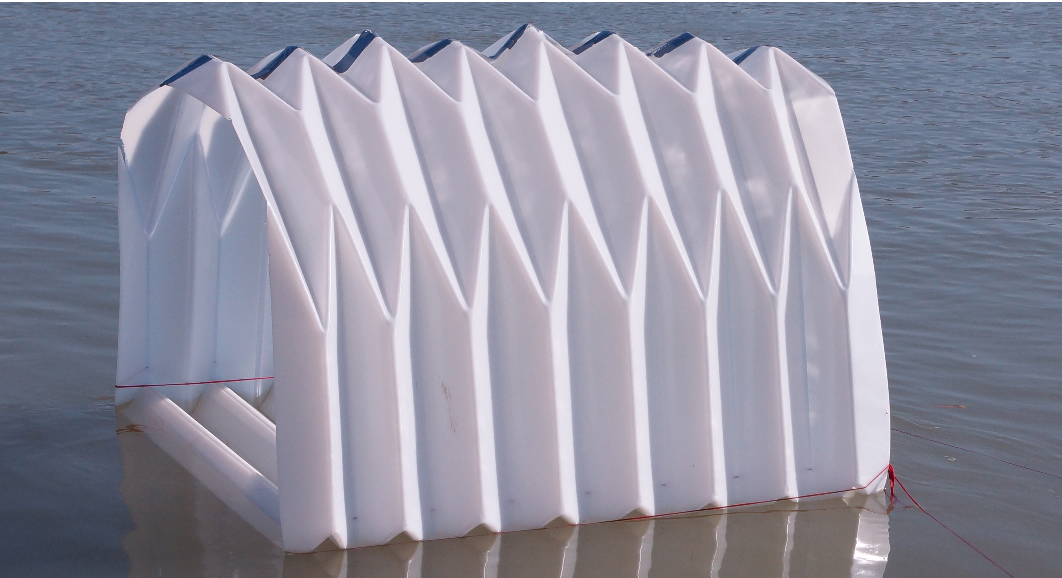
\includegraphics[width = 0.5\linewidth]{introduction/fig/OrigamiEx.png}
    \caption{Origami for disaster relief structure \cite{Tepa}}
    \label{fig:OrigamiEx}
\end{figure}


Furthermore the concepts of origami combined with the metamaterials provide a way for the structures which follow different energy pathways during deployment and contraction, which makes them highly desirable since they can be designed to resist immediate collapse by providing an energy barrier in their contraction pathway\cite{Zha}. This also adds to the reliability for use of deployable structures making their stability less dependent on locking mechanisms. In addition to this Origami can also be used for programming curvatures\cite{Dud}, and development of metamaterials\cite{Filip}.

In simple cases of pure origami based deployable hollow triangulated cylinders, based on the energy required the structures can be classified as easy-deploy-easy-collapse (requiring no or minimal energy for deployment as well as collapse) or hard-deploy-hard-collapse (requiring significant amount of energy for deployment as well as collapse). Easy-deploy-easy-collapse structures generate minimal strain in members of their equivalent bar and hinge model while hard-deploy-hard-collapse structure create large strains leading to even failure in case of conventional materials\cite{Zha,FilipBarandHinge}. The tubes can be designed to fall in one of the types by varying simple parameters which is shown in the next chapter.

\section{Deployable Structures and Metamaterials}
The domain of metamaterials which deals with materials having tunable stiffness forms a connection between metamaterials and deployable structure. Simplest instance of use of metamaterials in deployables is in the structures which have different energy paths for deployment and collapse, as explained earlier. Using a conventional material, if an element experiences compression during the process of deployment, it will experience tension while collapsing and usually the stiffness in tension as well as compression is same for materials and thus energy path followed is same for two deployment as well as collapse, however for material which exhibit different stiffness for tension and compression will have different profiles for two process and can lead to structures which deploy easily but offer resistance for collapsing and vice versa.\cite{Zha} 

Furthermore soft metamaterials and materials at the verge of instability have parameters which can be tuned to develop hinges and joints as part of elements engendering the possibility of a unified deployable systems without any external joints.\cite{Baardink489, Rock}

Design of metamaterials also draws from Origami, Mechanism, Topology, and form finding making a cohesive whole of all these ideas\cite{Filip, Rock}.


\section{Deployable Structures and Form Finding}
The concepts of form finding approach the topic of deployable structure from other direction. The ideas of form finding are usually applied in the reverse direction to determine the boundary conditions which will lead to the structure taking the desired shape. The deformations involved are usually large and material needs to be elastic during the entire process so that the structure can be deployed and collapsed a number of times, this provides another entry point for the application of metamaterials.

An example where this relationship is elicited is that of form finding in elastic gridshells. Initially planar elastic grid is actuated into a shell like structure by loading their extremities. It was observed that the resulting shapes are complex even for simple configuration and indicated the presence of multi-stable states and higher order modes in the actuated grid. However it is possible to parameterize these complex shape and by varying these parameters desired actuated shape can be obtained\cite{Baek75}.

\section{Deployable Structures and Elastic Bilayers}
In general nonuniform in-plane growth of thin sheets results in out of plane buckling. This process is responsible for several process in nature such as shaping of leaf and blooming of flowers. Generally, such sheets settle in residually strained configuration which is a local minima of the energetic cost of stretching and bending the sheet. Since it's a local minima, this state might not be unique. By solving the inverse problem one can design the layer such that it can be used to achieve any target surface shape from any reference shape\cite{va}. Similar to the case of form finding, this involves parameterizing the surface and solving the inverse problem.

\section{Deployable Structures and Topological Mechanics}
Topology involves the study of connectivity of different elements in a system and is essential to the idea of deployable structures. Topology plays an important role in determining the member connectivity in deployable trusses and folding motions of Origami and Kirigami\cite{Che}.

In addition to the deployable structures, It has a huge role in development of metamaterial\cite{Rock, Berto, Surj} and lattice mechanics\cite{Ma}. Topology can be used to control the mechanical properties of a material along an edge or around a localized defect, topological polarization of a network governs along with its variation and orientation define the rigidity of the network. The topology of the lattices can be varied to move between states with dramatically varying mechanical properties such as elastic modulus, wave characteristics and so on. 

\section{Deployable Structures and Lattices}
The deployable structure connects with the lattices at two level, on a trivial level, the lattices can be considered as a special kind of structure and mechanisms involved in such structures connect them directly with the ideas of deployable structure. Lattices require special attention owing to their periodic boundary conditions. Depending on the topology of lattice, actuation may propagate throughout the lattice or may cease within a few unit cells \cite{Neli}. Furthermore, it can be shown that static determinacy and kinematic determinacy can not exist in these structures concurrently \cite{Gues}. 

On a more elaborate level, Metamaterials connect the deployable structures with lattices since design of metamaterials requires realization and application of lattice mechanics and properties which is ultimately utilized for development of deployable structures. Lattice mechanics is essential to the development of metamaterials with unusual elastic modulus and phonon gaps.\cite{Ma}
\chapter{Models, Simulations and Findings}

%Check for mail with subject "Energy diagrams for hexagonal cell"

\section{Deployable Origami Tubes}
Two types of triangulated Origami tubes were developed and were tested for deployability. In accordance with the idea of energy profile based on the sum of two angles of the triangular units of the tubes easy-deploy-easy-collapse and hard-deploy-hard-collapse tubes were developed\cite{Zha}. 

The cylindrical tube is generated by joining two edges of the sheet show in the Fig~\ref{fig:AlphaBeta}. For the angles shown in Fig~\ref{fig:AlphaBeta}, if $\alpha + \beta < 90^{\circ}$ the tube is of the easy-deploy-easy-collapse (Fig~\ref{fig:EDEC}) type and if the sum is greater than $90^{\circ}$ i.e $\alpha + \beta > 90^{\circ}$ the mechanism is of hard-deploy-hard-collapse type(Fig~\ref{fig:HDHC}). It was observed from analysis of numerical model that for the hard-deploy-hard-collapse model ($\alpha = 50^{\circ}, \beta = 50^{\circ}$), the strain in equivalent bar hinge model would be of the order 20\% and hence the collapse is not possible in normal paper model. Also the hard-deploy-hard-collapse model carried significant lode before the paper model underwent local buckling at its creases.
\begin{figure}[htbp]
\centering
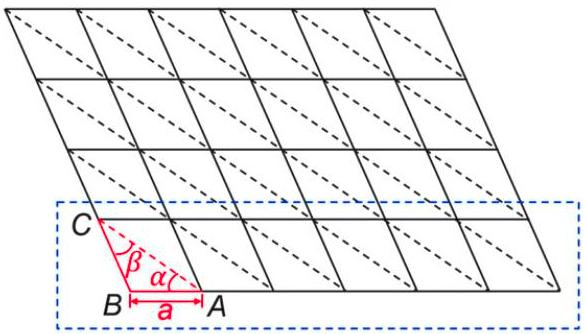
\includegraphics[width=0.6\linewidth]{introduction/fig/AlphaBeta.jpg}
\caption{Crease Pattern For Cylindrical Tube}
\label{fig:AlphaBeta}
\end{figure}

\begin{figure}
\centering
\begin{minipage}{.5\textwidth}
  \centering
  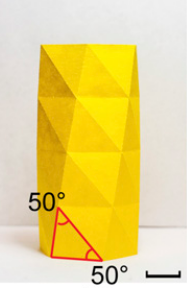
\includegraphics[width=.4\linewidth]{introduction/fig/HardDeploy.png}
  \captionof{figure}{Hard-Deploy-Hard-Collapse}
  \label{fig:EDEC}
\end{minipage}%
\begin{minipage}{.5\textwidth}
  \centering
  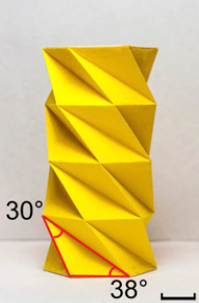
\includegraphics[width=.4\linewidth]{introduction/fig/EasyDeploy.png}
  \captionof{figure}{Easy-Deploy-Easy-Collapse}
  \label{fig:HDHC}
\end{minipage}
\end{figure}


\section{Energy Profiles}
The simulated energy profiles for the origami tubes are shown in the Fig~\ref{fig:EnergyProfile}. The simulation was performed for the equivalent bar hinge model.
\begin{figure}[htbp]
\centering
	\subfigure[Easy-Collapse-Easy-deploy energy profile ]{
	\centering
		\label{fig:ECEDEP}
        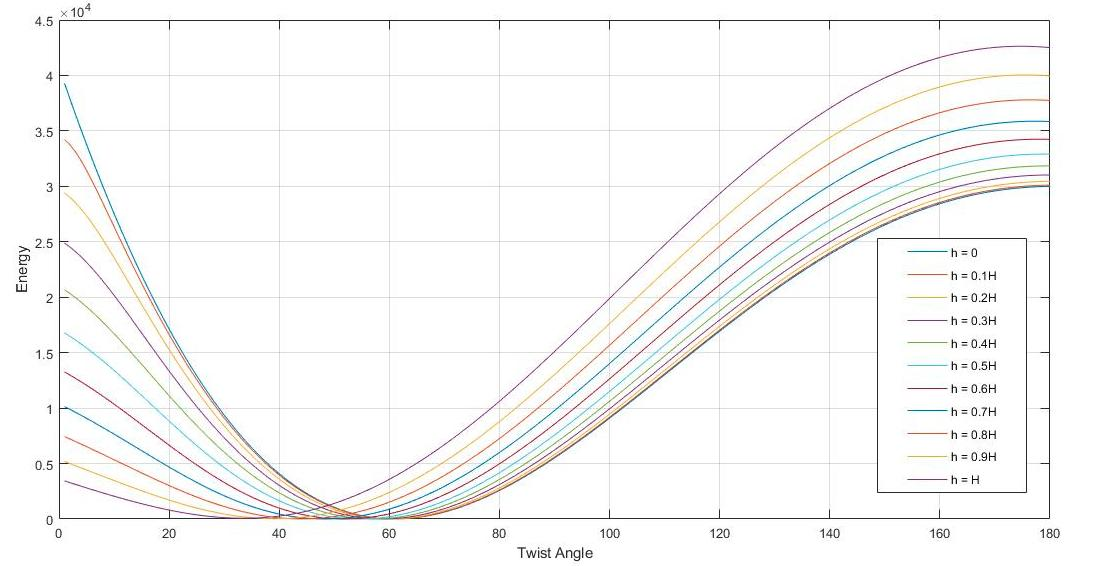
\includegraphics[width=1\linewidth]{introduction/fig/EDEC.jpg}}
	\subfigure[Hard-Collapse-Hard-deploy energy profile]{
	\centering
		\label{fig:HCHDEP}
		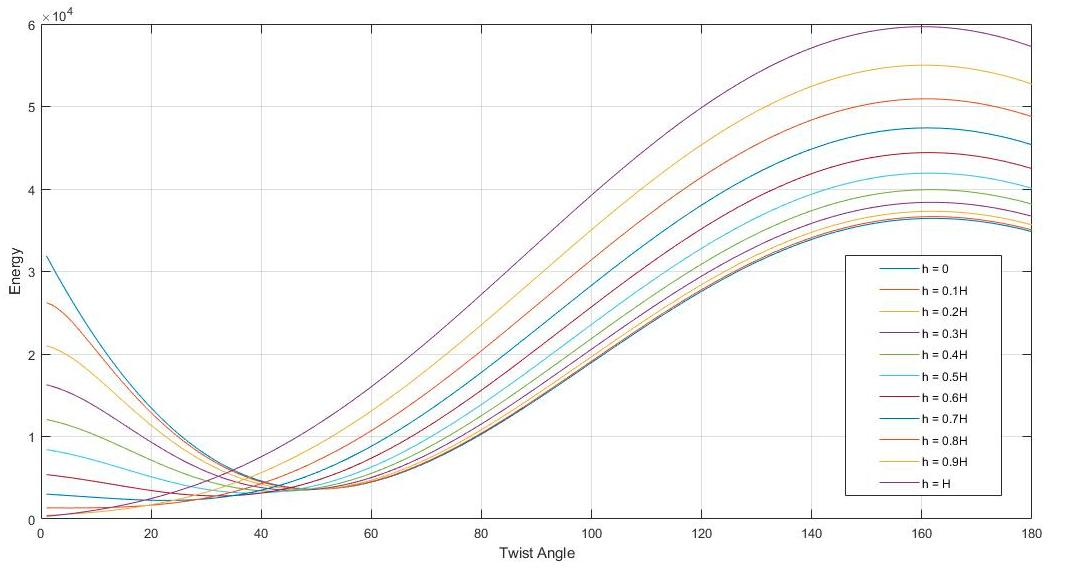
\includegraphics[width=1\linewidth]{introduction/fig/HDHC.jpg}}
	\caption{Energy Profiles}
	\label{fig:EnergyProfile}
\end{figure}

As it can be seen from the energy profile obtained by computing energy in the structure at various stages of deployment, the easy-deploy-easy-collapse structure presents negligible energy barrier as opposed to the hard-deploy-hard-collapse structure in which significant energy barrier is present for process of deployment as well as collapse. 

Using metamaterials, a structure which presents no energy barrier during deployment but exhibits resistance to collapse can be developed. This will provide the reliability to the deployable structure without being dependent on locking mechanisms for its stability.

\section{Lattices}
The current work is directed towards developing a Julia program which can generate lattices and predict the behavior of lattice using simple spring ball models. Currently the effort is directed toward developing a program which can create finite lattices with provided boundary conditions. Small displacements are provided in direction normal to lattice to induce out of plane curvatures. A sample rectangular lattice generated using the Julia program is presented in the Fig~\ref{fig:RectLattice}.
\begin{figure}[htbp]
    \centering
    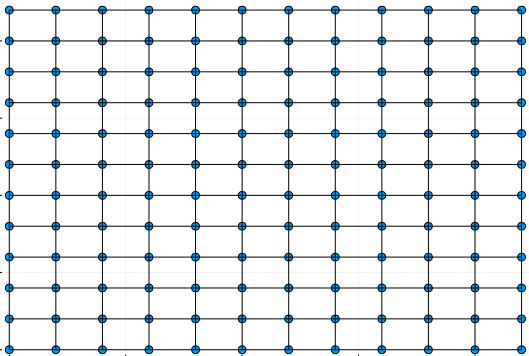
\includegraphics[width = 1\linewidth]{introduction/fig/lattice.png}
    \caption{Rectangular lattice}
    \label{fig:RectLattice}
\end{figure}{}
\chapter{Future Work}

While current work has contributed towards modelling plates using spring ball system through an energy minimization. In addition to helping in prediction of deflection and other relevant quantities for complex loading, shape and other conditions, this project can be continued to study the following promising fields some of which pave the way for deployable Structures while others guide towards the development of metamaterials with interesting mechanical properties.

\section{Form Finding}
This will involve studying the shapes that lattice takes under different stimulus such tweaking the spring lengths, varying stiffness of the springs, providing pre-tensions in the spring and so on. This will be used to induce curvature, morphing into different shapes and so on.\cite{DU2020103370}\cite{Jones_2015}

\begin{figure}[!htbp]
    \centering
    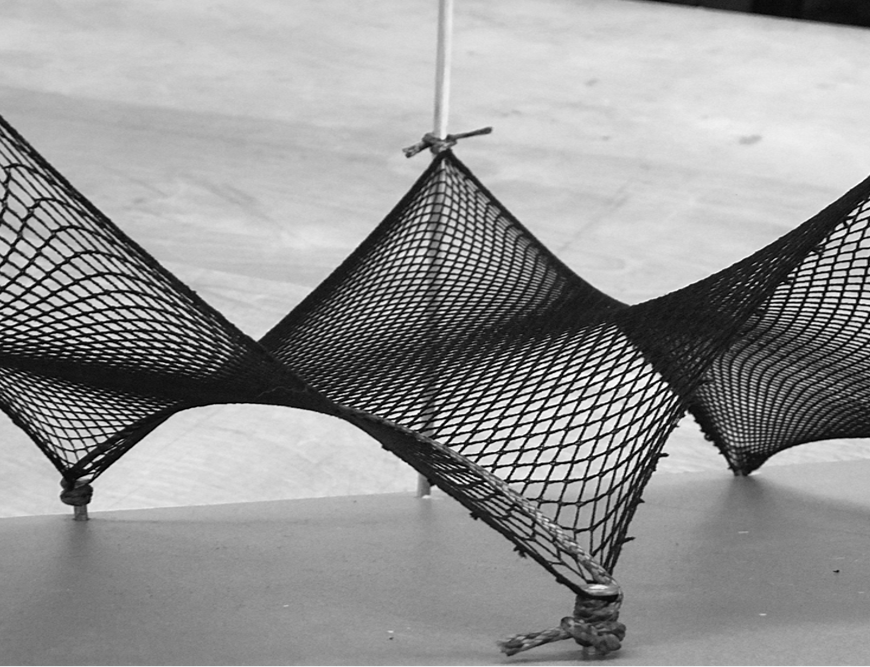
\includegraphics[width = 1\textwidth]{Figures/form_finding.png}
\end{figure}

\section{Vibration Modes \& Wave Propagation}
Using the concepts of reciprocal lattice in addition to the program, the phonon modes of the structure and other relevant lattice characteristics can be determined which will provide insights into the vibrational modes of lattice and wave propagation characteristic of the lattice. This model will aid in understanding the effect of selective pre-stress and topology on the static and dynamic property of the model.\cite{Ma}
\begin{figure}[!htbp]
    \centering
    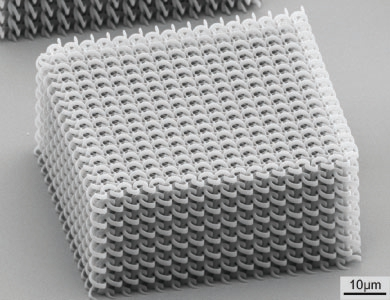
\includegraphics[width = 1\textwidth]{Figures/wave_prop_metamterials.jpg}
\end{figure}

\appendix
\chapter{Non Linear Behavior of Horizontal Spring System under Vertical Load}

Fig~\ref{fig:Non_linear_system} below represents the system used for carrying out the study. The plot shown in fig~\ref{fig:Non_linear_system_plot} present the response of the system. The reaction is normalized by stiffness of the linear springs and the displacement are normalized by the natural lengths of the spring.

\begin{figure}[!htbp]
    \centering
    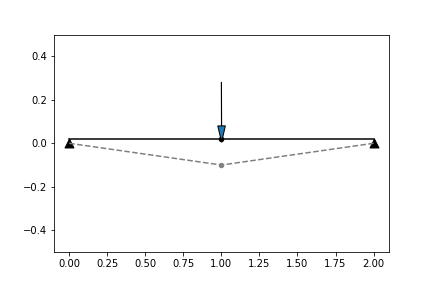
\includegraphics[width = 0.5\textwidth]{Figures/non_linear_spring_behavior.png}
    \caption{Spring system for Non-Linear behavior}
    \label{fig:Non_linear_system}
\end{figure}

\begin{figure}[!htbp]
    \centering
    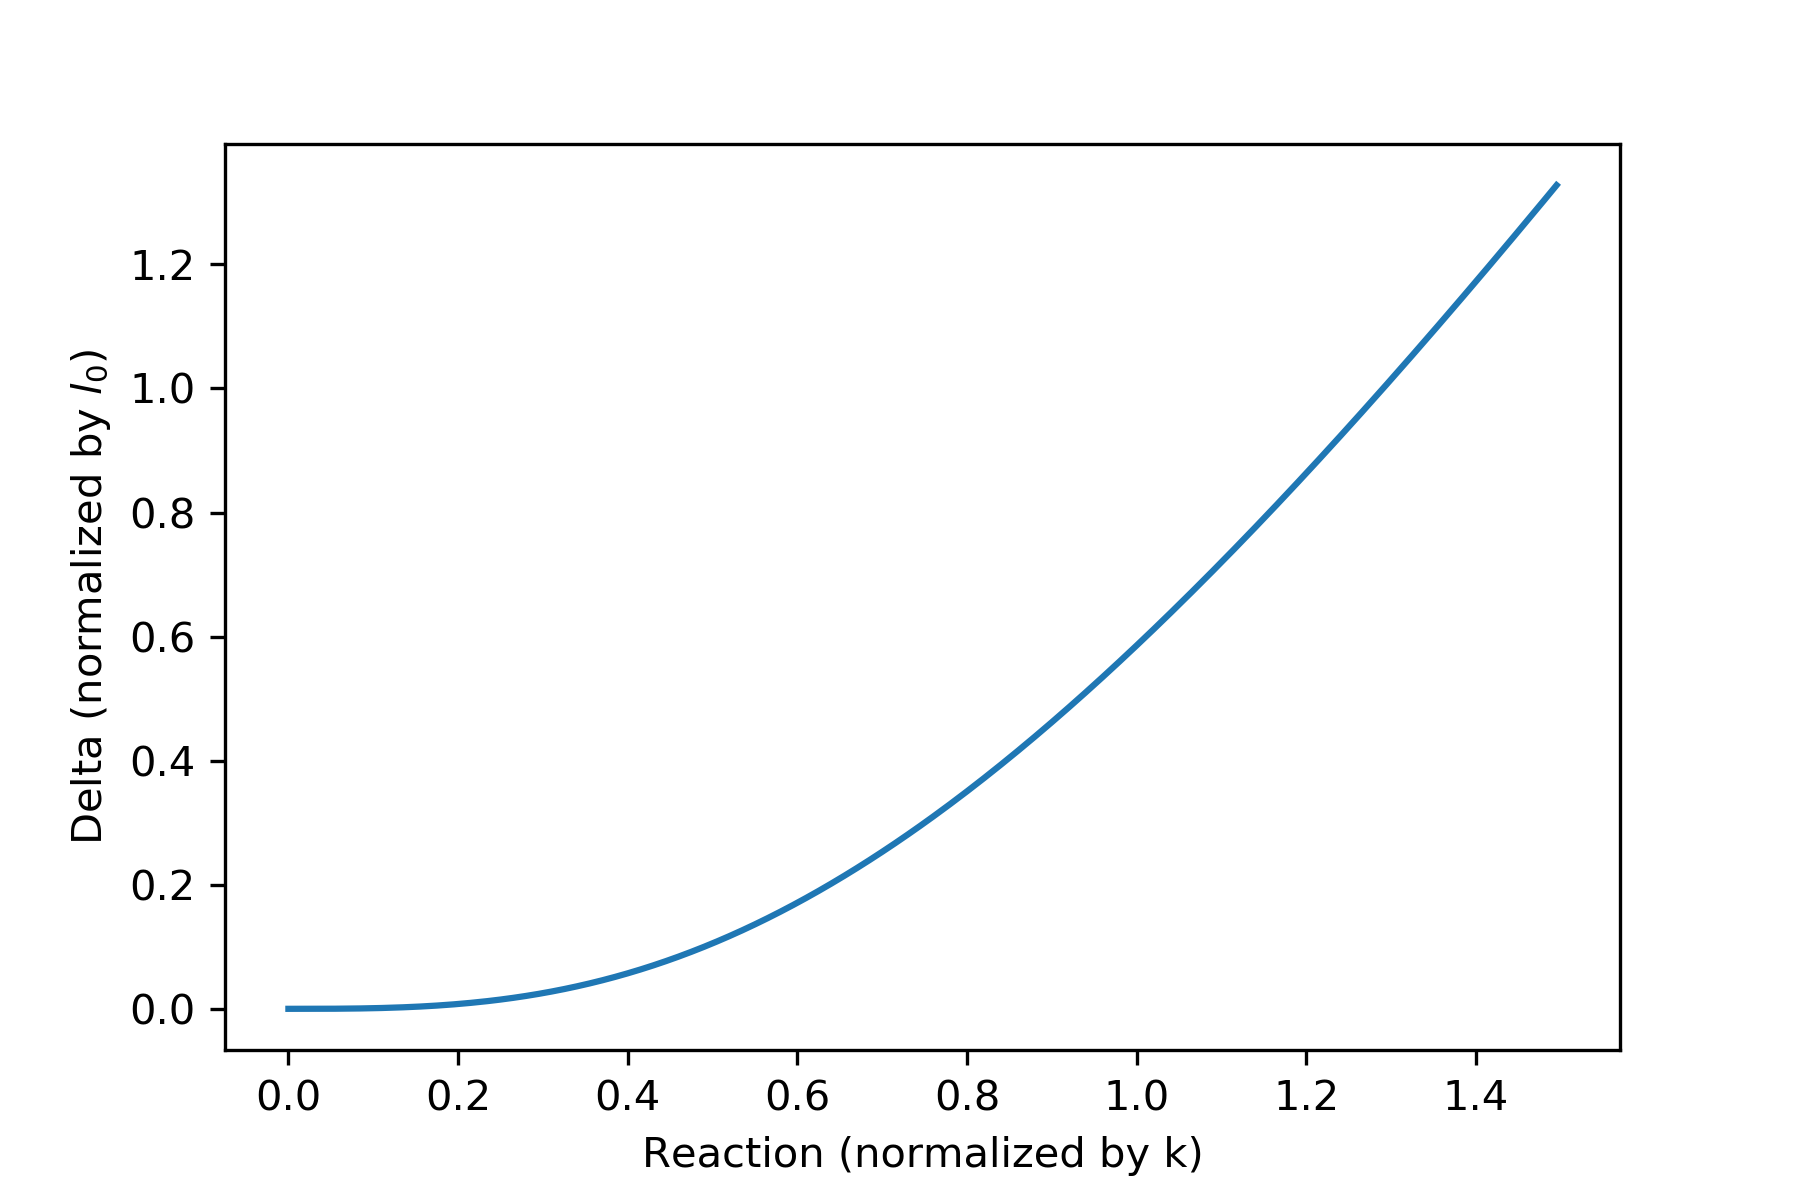
\includegraphics[width = 0.5\textwidth]{Figures/spring_response.png}
    \caption{Response of the Spring System}
    \label{fig:Non_linear_system_plot}
\end{figure}

As it can be seen from the response, initially the spring only offers second order reaction for small deflections at centre. With reference to the models presented in the project, this explains the crushing of the vertical springs at high loading since horizontal spring system offers no vertical reaction to the applied loading at the start. Adding body diagonals helps in distribution of the concentrated load and hence Model 3 is more stable performance under loading. 



\bibliographystyle{unsrt}
\bibliography{bibs/sample}
\addcontentsline{toc}{chapter}{Bibliography}

\end{document}